\documentclass[a4paper]{article}

\usepackage{array}
\usepackage{placeins}
\usepackage{listings}
\usepackage{hyperref}
\usepackage{enumitem}
\usepackage{todonotes}

\usepackage{hopsantut}

\begin{document}
\maketitle{Optimizing Models With modeFRONTIER}

\section*{Legal Notice}
modeFRONTIER is the property of
Vi är inte affilierade med dem

\section*{Introduction}
\todo[inline]{Skriv något!}

\section*{Requirements}
modeFRONTIER 4.5.3
Hopsan version 0.6.7 or later
Tutorialen är skriven för Windows, med fungerar även i Linux med vissa modifikationer

%\icon{0}{gfx/Hopsan-ExportSimulink.png}{Export model to Simulink S-function}


\section*{Optimize using final values only}
\todo[inline]{Skriv något!}

\begin{enumerate}
\tutitem{Preparations}
%- Skapa en ny (tom) mapp
%- Öppna Position Servo-exemplet
%- Lägg till integrator (bild)
%- Spara i mappen som PositionServo.hmf
%- Öppna cmd (start meny -> run -> cmd)
%- Gå till mappen
%- Kör HopsanCLI med följande kommandon för att öppna modellen, simulera och generera filer för parametrar och variabler:
%  %"c:\Program Files (x86)"\hopsan\bin\HopsanCLI --hmf PositionServo.hmf --simulate hmf --resultsFinalCSV resultsFinal.csv  --parameterExport parameters.csv"
 
\tutitem{Build the modeFRONTIER project}
%- Öppna modeFRONTIER
%- Skapa ett nytt projekt och spara det i mappen som skapades ovan
%Processer:
%- Scheduler
%- DOS Batch Script
%- Logic End
%Input:
%- Input File
%- 2x Input Variable
%- Support File
%Output:
%- Output File
%- Output Variable
%- Design Objective

\begin{center}
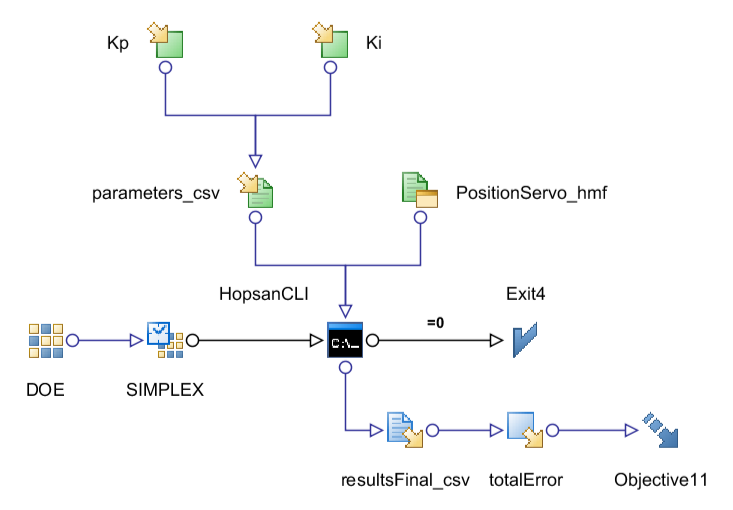
\includegraphics[scale=0.56]{gfx/modefrontier/model_final.png}\\
\end{center}

\tutitem{Specify input parameters}
%0 < Kp < 0.01
%0 < Ki < 0.005

\tutitem{Configure the input parameter file}
%- Dubbelklicka på input file-noden
%- Sätt "Input File Node Name" till "parameters_csv"
%- Bläddra till mappen du skapade
%- Öppna parameters.csv
%- Markera Kp i listan längst ner
%- Bläddra fram raden som börjar med "PositionServo$GainP#k#Value"
%- Markera det numeriska värdet sist på raden
%- Högerklicka -> Insert Variable
%- Markera Ki i listan längst ner
%- Bläddra fram raden som börjar med "PositionServo$GainI#k#Value"
%- Markera det numeriska värdet sist på raden
%- Högerklicka -> Insert Variable
%- Klicka på "Ok" två gånger för att stänga dialogerna

\tutitem{Configure the Hopsan model file}
%- Dubbelklicka på Support File-noden
%- Sätt "Support File Node Name" till "PositionServo_hmf"
%- Klicka på "Add file"
%- Välj "PositionServo.hmf"
%- Klicka på Ok

\tutitem{Specify the output variable}
%- Dubbelklicka på Output Variable-noden
%- Sätt "Name" till "totalError"
%- Klicka på Ok

\tutitem{Configure the output file}
%- Dubbelklicka på output file-noden
%- Sätt "Output File Node Name" till "resultsFinal_csv"
%- Klicka på "Open Output File"
%- Välj "resultsFinal.csv"
%- Bläddra till raden som börjar med "PositionServo$totalError#out#Value"
%- Klicka på totalError längst ner
%- Markera texten "PositionServo$totalError#out#Value"
%- Högerklicka -> Relative Position
%- Markera det numeriska värdet sist på raden
%- Högerklicka -> Select Relative
%- Klicka på Ok två gånger

\tutitem{Define the objective function}
%- Dubbelklicka på "Design Objective"-noden
%- Ändra "Maximize" till "Minimize"
%- Klicka på Ok

\tutitem{Write a script for controlling HopsanCLI}
%- Dubbelklicka på script-noden
%- Sätt "Name" till "HopsanCLI"
%- Klicka på "Edit DOS Batch Script"
%- Skriv följande tre rader:
%  SETLOCAL
%  SET PATH=%PATH%;C:\"Program Files (x86)"\Hopsan\bin
%  HopsanCLI --hmf PositionServo.hmf --simulate hmf --resultsFinalCSV resultsFinal.csv --parameterImport parameters.csv
%- Klicka på Ok två gånger

\tutitem{Choose initial distribution and algorithm}
%- (skriv att vilka inställningar som helst kan användas, dessa är bara exempel)
%- Dubbelklicka på DOE-noden
%- Välj "Random" under "Space Fillers" till vänster
%- Klicka på "Add DOE Sequence"
%- Klicka på Ok
%- Dubbelklicka på Scheduler-noden
%- Välj "Simplex" under "Heuristic Optimizers"

\tutitem{Run an optimization}
%- Spara modellen
%- Gå till "Run Analysis"-läge
%- Klicka på den gröna pilen uppe till höger
\end{enumerate}



\section*{Optimizing using full variable export}
\todo[inline]{Skriv något!}

\begin{enumerate}
\tutitem{Save a copy of the model}
%- Spara modellen från metod 1 i samma mapp men med nytt namn

\tutitem{Generate output variable file}
%- Öppna kommandofönstret och gå till mappen
%- Kör HopsanCLI med följande kommandon för att öppna modellen, simulera och generera en fil för variabler:
%    "c:\Program Files (x86)"\hopsan\bin\HopsanCLI --hmf PositionServo.hmf --simulate hmf --resultsFinalCSV resultsFinal.csv  --parameterExport parameters.csv"

\tutitem{Modify the HopsanCLI script}
%- Dubbelklicka på skript-noden
%- Klicka på Edit DOS Batch Script
%- Ändra skriptet till följande:
%  SETLOCAL
%  SET PATH=%PATH%;C:\"Program Files (x86)"\Hopsan\bin
%  HopsanCLI --hmf PositionServo.hmf --simulate hmf --resultsFullCSV resultsFull.csv --parameterImport

\tutitem{Rebuild the project}
%- Ta bort output file-noden
%- Lägg in en Output Template-nod och en Calculator-nod mellan script-noden och exit-noden
%- Lägg in en Transfer File-nod mellan Script-noden och Output Template-noden
%- Lägg in två Output Vector-noder mellan Output Template-noden och Calculator-nodne
%- Koppla ihop Calculator-noden med den redan existerande totalError-noden

\begin{center}
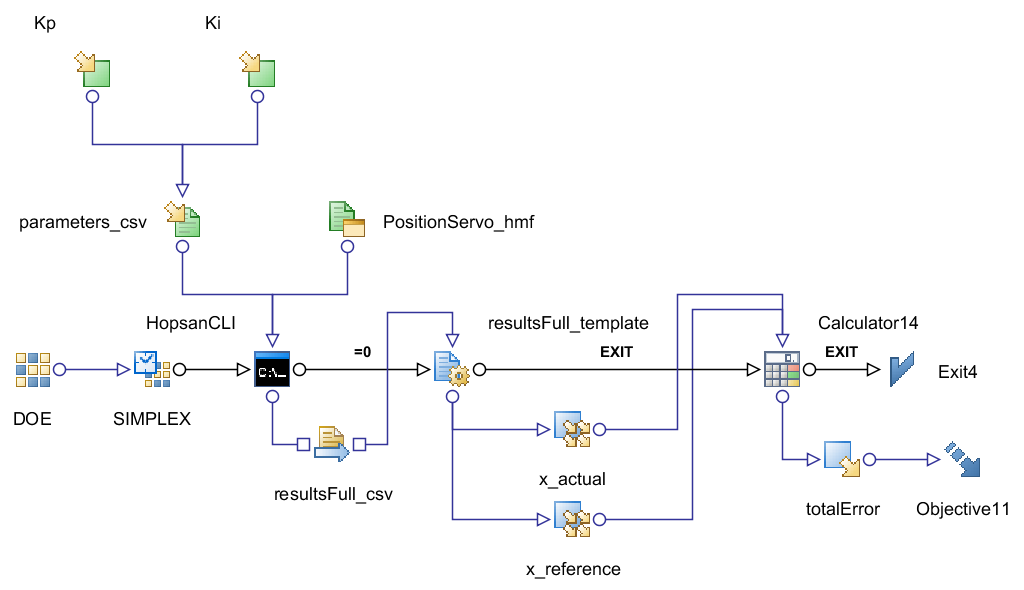
\includegraphics[scale=0.56]{gfx/modefrontier/model_full.png}
\end{center}


\tutitem{Specify output variables}
%- Dubbelklicka på en av OutputVector-noderna
%- Sätt name till "x_actual"
%- Sätt Size till 2048
%- Klicka på Ok
%- Dubbelklicka på den andra av OutputVector-noderna
%- Sätt name till "x_reference"
%- Sätt Size till 2048
%- Klicka på Ok

\tutitem{Configure the output varible file}
%- Dubbelklicka på Transfer File-noden
%- Sätt Transfer File Node Name till "resultsFull_csv"
%- Klicka på "Add File"
%- Skriv "resultsFull.csv" 
%- Klicka på Ok två gånger

\tutitem{Configure the data mining}
%- Dubbelklicka på Output Template-blocket
%- Sätt Output Template Node Name till "resultsFull_template"
%- Klicka på "Edit Output Template"
%- Bläddra till mappen, välj "resultsFull.csv"
%- Klicka på x_actual längst ner
%- Bläddra fram raden som börjar med "PositionServo$Position_Sensor#out#Value"
%- Markera texten, högerklicka -> Add Rule For -> x_actual
%- Markera texten igen, högerklicka -> Set Anchor -> x_actual
%- Kryssa ur kolumn 1, 2, 3 och 4 till vänster
%- Klicka på x_reference längst ner
%- Bläddra fram raden som börjar med "PositionServo$Step#out#Value"
%- Markera texten, högerklicka -> Add Rule For -> x_reference
%- Markera texten igen, högerklicka -> Set Anchor -> x_reference
%- Kryssa ur kolumn 1, 2, 3 och 4 till vänster
%- Klicka på Ok två gånger

\tutitem{Define the objective function calculation}
%- Dubbelklicka på Calculator-blocket
%- Sätt "Name" till "objective_function"
%- Klicka på "Edit Calculator Expression"
%- Skriv följande: 
%  "totalError = sum(abs(subtract(x_actual,x_reference)))"
%- Klicka på Ok två gånger
  
\tutitem{Save the model and run an optimization}

\end{enumerate}

\end{document}